%% This chapter discusses the technologies and the architecture
\chapter{Architecture \& Technology Overview}

In this chapter, I will briefly discuss the frameworks used in the project, followed by how well they served their intended purpose as well as how they work in tandem as a complete system.

%%%%%%%%%%%%%%%%%%%%%%%%%%%%%%%%%%%%%%%%%%%%%%%%%%%%%%%%
%% List the tehnologies that were used.
\section{Technologies Used}

\textbf{JavaScript} is the base programming language in the project. However, each part of the system is built using a suitable framework. In this section, I will only list the frameworks.

\subsection{Client Application}

\textbf{Ionic} \cite{ionic-site} is used as the 'app' framework. It provides the GUI components as HTML and CSS and plug-ins for platform specific support for mobile  features like camera, calendar etc. from \textbf{Cordova} \cite{ngcordova-site}. As for the JavaScript part of the application, it uses an opinionated framework, \textbf{AngularJS} \cite{angular-site}, to provide interactivity and navigation.

\subsection{Server Application}

I used \textbf{NodeJS} \cite{nodejs-site}, a non-blocking JavaScript runtime, and \textbf{Express} \cite{expressjs-site}, an unopinionated framework, to build the server. \textbf{MongoDB} \cite{mongodb-site}, a NoSQL database, was used for storage.

\subsection{Test Suits}

\textbf{MochaJS} \cite{mocha-site}, a JavaScript test framework, was used as the automated test runner and the assertion library was \textbf{ShouldJS} \cite{shouldjs-site}.

\subsection{Cloud Platform}

The server was hosted on \textbf{Heroku} \cite{heroku-site}, a PaaS (Platform-as-a-Service), while \textbf{mLab} \cite{mlab-site} hosted the database.

%%%%%%%%%%%%%%%%%%%%%%%%%%%%%%%%%%%%%%%%%%%%%%%%%%%%%%%%


%%%%%%%%%%%%%%%%%%%%%%%%%%%%%%%%%%%%%%%%%%%%%%%%%%%%%%%%
%% How well did these perform from expected
\section{Applicability of Technology}

In this section, I will discuss how the aforementioned frameworks helped in development.

\subsection{Ionic \& AngularJS}

Ionic provides HTML 5 and CSS built components like in Figure \ref{fig:ionic-comp-ex}. These are easily customisable and provides great usability on mobiles. Using the CLI (Command Line Interface), I easily added plug-ins  (\texttt{ionic add <plugin>}), different platform support (\texttt{ionic add <platform>}) and generated platform specific installable app (\texttt{ionic <build || run> <platform>}) without writing any native code.\\

\begin{figure}[h]
    \centering
    \begin{subfigure}[b]{0.3\textwidth}
        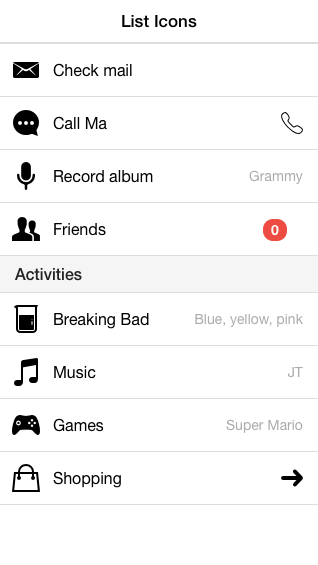
\includegraphics[width=\textwidth]{ionic-a}
    \end{subfigure}
    ~
    \begin{subfigure}[b]{0.3\textwidth}
        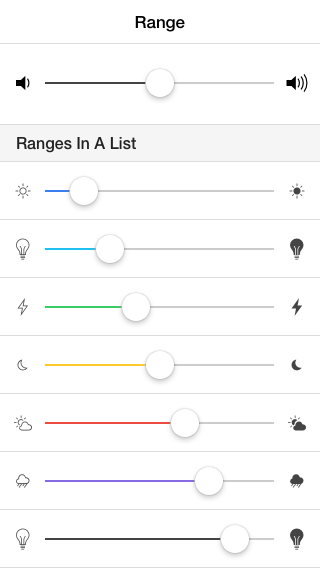
\includegraphics[width=\textwidth]{ionic-b}
    \end{subfigure}
    ~ 
    \begin{subfigure}[b]{0.3\textwidth}
        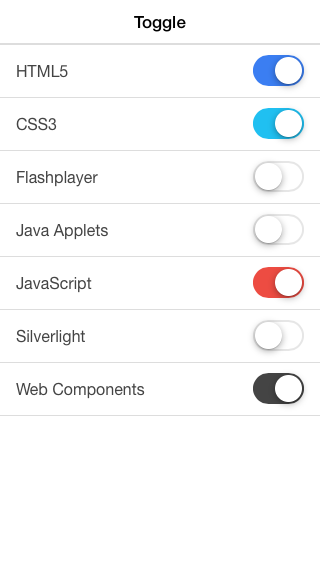
\includegraphics[width=\textwidth]{ionic-c}
    \end{subfigure}
    \caption{Ionic Component Examples}\label{fig:ionic-comp-ex}
\end{figure}

I structured the code in MVC (Model View Controller) pattern and created navigation between views using AngularJS. Angular's \textit{directives} bind a view with the underlying data structure, for example - bind a table to a list, so updating views is made very easy.

\subsection{NodeJS \& MongoDB}

NodeJS is completely asynchronous, so it can utilise IO operations (database query) very efficiently (compared to Apache for example) and serve magnitudes of more clients (Figure \ref{fig:node-comp-ex} \cite{tomislav-site}), despite being single-threaded. In fact, it is 2.5 magnitudes faster than PHP and cpu-memory efficient. As the system is meant to handle many users simultaneously, it is highly advised to use Node to handle such real-time communication, specially in tandem with hybrid platforms \cite{Chaniotis:2015}.\\

\begin{figure}[h]
    \centering
    \begin{subfigure}[b]{0.45\textwidth}
        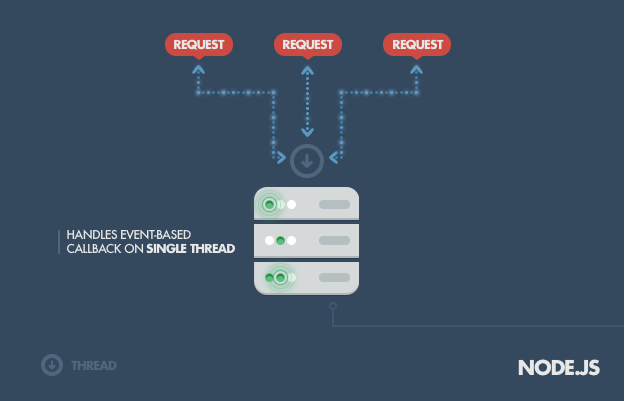
\includegraphics[width=\textwidth]{node-a}
    \end{subfigure}
    ~
    \begin{subfigure}[b]{0.45\textwidth}
        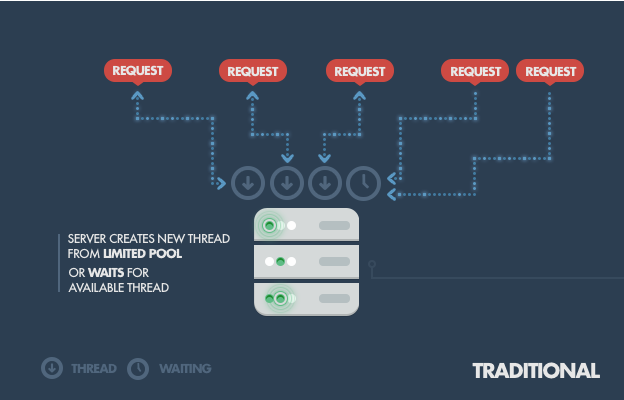
\includegraphics[width=\textwidth]{node-b}
    \end{subfigure}
    \caption{NodeJS}\label{fig:node-comp-ex}
\end{figure}

MongoDB is schema-less and document driven. As a NoSQL database, it is highly scalable and can handle unstructured data, multimedia and social-media content efficiently \cite{cornelia:2015}. Indeed, Mongo's flexibility was necessary for fast prototyping and suitable for the app's intention.

\subsection{Heroku \& mLab}

Out of the well known PaaS such as Bluemix \cite{bluemix-site}, Openshift \cite{openshift-site}, AppEngine \cite{gae-site} etc., Heroku is by far the easiest to use (to get started and deploy), in my opinion, and has the best community support. A PaaS takes care of infrastructure tasks like hosting a server, scaling it etc. So, I could focus more on development. As for mLab, it is a generic MongoDB hosting site with free usage upto 500 MB and easily integrated with Heroku.

\subsection{Issues}
\label{subsec:issues}

There were some issues that could not be avoided with the selection of technology - 

\begin{description}

	\item [GCM] (Google Cloud Messaging) \cite{gcm-site} is the only entity that can send push notification to an Android phone (even though intermediate frameworks, e.g. Ionic Push, can be involved). While it is possible to verify if a request for notification has been accepted, when it gets delivered cannot be controlled in any way. Often a notification will be found as sent, but it will not actually arrive for hours. The probable reason is that, I used a \textit{free} GCM service rather than a \textit{paid} one.
	
	\item [Base64] images \cite{base64-site} are ASCII encodings of binary image files. Although, Amazon S3 \cite{s3-site} is the preferred service to store images, it is not free. So, I stored images as very large strings in MongoDB. This should be avoided a production-ready app.
	
\end{description}

%%%%%%%%%%%%%%%%%%%%%%%%%%%%%%%%%%%%%%%%%%%%%%%%%%%%%%%%


%%%%%%%%%%%%%%%%%%%%%%%%%%%%%%%%%%%%%%%%%%%%%%%%%%%%%%%%
%% Discuss how the technologies work together
\section{Architecture}

%%%%%%%%%%%%%%%%%%%%%%%%%%%%%%%%%%%%%%%%%%%%%%%%%%%%%%%%

In this section I will discuss how different parts of the project comes together. Figure \ref{fig:archi} is the complete architecture diagram which will be referred to in the following sections.

\begin{figure}[h]
    \centering
    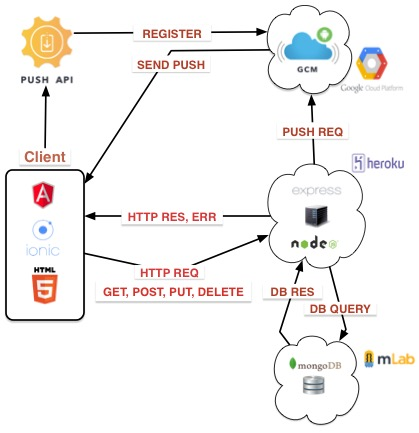
\includegraphics[height=0.7\textwidth]{architecture}
    \caption{System Architecture}\label{fig:archi}
\end{figure}

\subsection{Client-Server Communication}

The Ionic client app makes requests to the NodeJS server on Heroku to retrieve/create/update/delete various data artefacts. These requests are authorised by the \textit{PassportJS Local Strategy} (by unique username-password, rather than a social network). The server then asynchronously handles each request.

\subsection{Server-Databse Communication}

The server contacts the MongoDB database on mLab asynchronously (for which it has a key) for each client request. After the results reach the server, it asynchronously passes them to the Client. The client thus never directly contacts the database.

\subsection{Push Notification}

When the app is opened on a mobile first time, Client sends a GCM registration request via the Ionic Push API. This API registers the app, sends back a token to the client. Finally, the client sends the token to the server and it, in turn, saves it on mLab. In future, an event may be triggered on the server (e.g. new offer from a user) which may require a push notification to one-or-more clients. It sends a request to the GCM server to send a notification to the given tokens. GCM takes care of the actual sending of the notification.